\section{Introduction}
\setlength{\parindent}{2em}
\subsection{Background} % 背景
\indent As the earth's resources become increasingly scarce and the population continues to grow, human civilization is facing unprecedented sustainable development challenges. As the closest celestial body to the earth, the moon is rich in helium-3, titanium, iron and other mineral resources, as well as its strategic value as a springboard for deep space exploration. It is a key target for international space agencies to compete for layout.

\indent However, traditional space transportation systems using rocket transportation have significant bottlenecks. Currently, according to SpaceX data, the cost of sending a 1 kilogram payload into low-Earth orbit is about US\$2,720, and the cost of reaching the lunar surface is even higher. This high-cost, low-frequency transportation mode severely restricts the construction of large-scale space infrastructure. At the same time, this solution also seriously affects the earth's ecological environment due to the harmful gas emissions produced by the fuel.

\indent In contrast, the space elevator system has shown breakthrough potential as a revolutionary space transportation infrastructure. The system uses the balance between the centrifugal force of the Earth's rotation and gravity to set a vertex anchor point in the geosynchronous orbit 35,786 kilometers above the equator, and connects to ground ports through a 100,000-kilometer-long super-strong material tether to form a "space highway." Compared with traditional rockets, space elevators use electricity as a power source and can theoretically achieve large-scale material transportation with nearly zero carbon emissions, reducing unit transportation costs to less than one thousandth of traditional methods.

\indent This topic focuses on the envisaged plan to colonize the moon with 100,000 people in 2050. It analyzes the time cycle and economic cost of transportation of engineering materials in the early stages of lunar base construction, and the different transportation options that can be adopted for the water demand of the base after residents move in. Then, it comprehensively considers the environmental impact of different transportation options and provides different transportation options.

%\subsection{Literature Review} % 文献综述


\subsection{Restatement of the Problem} % 问题重述

\textbf{Problem1}:
It is estimated that the construction of a lunar colony of 100,000 people will require 100 million tons of materials. Under ideal conditions (no rocket launch failure, no tether shaking), three different options are adopted:
\begin{itemize}
  \item a:Three galactic ports using only space elevators
  \item b:Traditional solution using only ten Earth rocket launch systems
  \item c:A combination of two transport systems
\end{itemize}

This article will establish a mathematical model to calculate the transportation costs and time required for these three different options.

\textbf{Problem2}:
Expand the model of Question 1 to consider the impact of non-ideal factors on the transportation plan, that is, consider factors such as cable shaking of the space elevator system, elevator damage, and launch failure factors of the rocket transportation system. Due to these non-ideal factors, the annual carrying capacity of both transportation systems, as well as the unit transportation costs, will be affected. These effects are combined in the model of Question 1 to obtain the adjusted transportation plan.

\textbf{Problem3}:
After the lunar colony is completed and operated, what is the total water demand for a population of 100,000 and its distribution? A mathematical model is established to analyze this problem. Combined with the transportation system model of questions 1 and 2, a water delivery plan with optimal additional costs and timing is obtained on the premise of ensuring water supply for the colony.

\textbf{Problem 4:}
During the process of transporting materials, launching rockets will inevitably have an impact on the earth's environment. However, the earth's environment can only bear limited pollution. This impact will be taken into consideration in the model to re-formulate the material and water resources transportation plan for the realization of a 100,000-person lunar colony base.


\subsection{The Description of the Problem} % 问题描述

\textbf{Problem1}:
The scene in question 1 is set against the background of the initial construction of the lunar colony. Humanity has built a complete space elevator system, which can transport supplies to the moon through the Galaxy Port, and can also use ground rocket launch systems to transport supplies to the lunar base. Under the assumption that both the rocket launch and the space elevator system work under ideal conditions (no capacity loss, no additional cost), three transportation options are used: three galactic ports relying only on the space elevator system, traditional rocket launch using only existing bases, or a combination of the two methods. The time and economic costs required for different options are modeled and analyzed. Among them, in the combination scheme of the two methods, in order to solve the comprehensive optimization of time and economy and analyze the rocket launch arrangement, the multi-objective Pareto optimization model can be used for analysis. 
At the same time, considering the possible decline in rocket manufacturing costs, the annual decay coefficient of rocket manufacturing is introduced based on Wright's law, and a rocket cost iteration model is added to Plan C to optimize the plan.

\textbf{Problem2}:
The ideal assumption of Question 1 ignores the inherent risks of the space transportation system: the ultra-long cable of the space elevator is affected by orbital disturbance and mechanical wear, and there are problems such as cable shaking and equipment failure; traditional rocket launches are affected by weather and technical complexity, and face risks such as launch failure and reduced launch site efficiency. Such non-ideal factors will directly lead to capacity attenuation, cost increase and construction period extension. It is necessary to quantify the impact of faults and correct the original model to ensure that the solution has reliability and anti-interference capabilities in actual engineering scenarios. 
Abstract faults can be converted into quantifiable coefficient indicators to build capacity attenuation and cost addition models. Embed non-ideal parameters into the multi-objective optimization model of Problem 1, recalculate the time and cost of the three types of options, generate the modified Pareto front, and obtain the adjustments of each option under non-ideal conditions.

\textbf{Problem3}:
The total water demand after the 100,000-person lunar colony completes operations can be based on existing data from the International Space Station (ISS), Biosphere 2, etc., and a per capita daily water flux model can be constructed based on scenarios. At the same time, in order to maximize the utilization of water resources, a water recycling system must be considered. Then, the water demand, recycling efficiency and loss rate of each scenario are integrated to calculate the annual net water resource deficit (i.e. the annual water resource demand of the base). Embed the net supply demand into the early transportation model, compare the costs, capacity matching, and long-term operation and maintenance resilience of the three types of transportation routes, and introduce the redundant design idea of ​​"main transportation + backup".

\textbf{Problem 4:}
Large-scale Earth-to-Moon transportation will have a cumulative impact on the Earth's environment. Among them, the source of pollution can be considered to be only the ground rocket launch system, while the space elevator system has zero emissions and no pollution during transportation. First, the environmental cost of the transportation solution needs to be quantified. A composite environmental impact equivalent can be constructed based on the life cycle assessment (LCA) method and the environmental damage weight of multiple types of pollutants can be integrated. Secondly, the earth's environmental pollution carrying threshold can be derived. Based on the stratospheric aerosol steady-state load theory, the maximum annual number of rocket launches that the earth can withstand can be physically derived. Finally, the environmental impact is regarded as the third goal, embedded in the original time-cost optimization model, using the atmospheric carrying capacity as a hard constraint, correcting the upper limit of rocket launch frequency, and screening the three-dimensional Pareto optimal solution.

\subsection{Our Work} % 我们的工作
\begin{figure}[htbp]
  \centering
  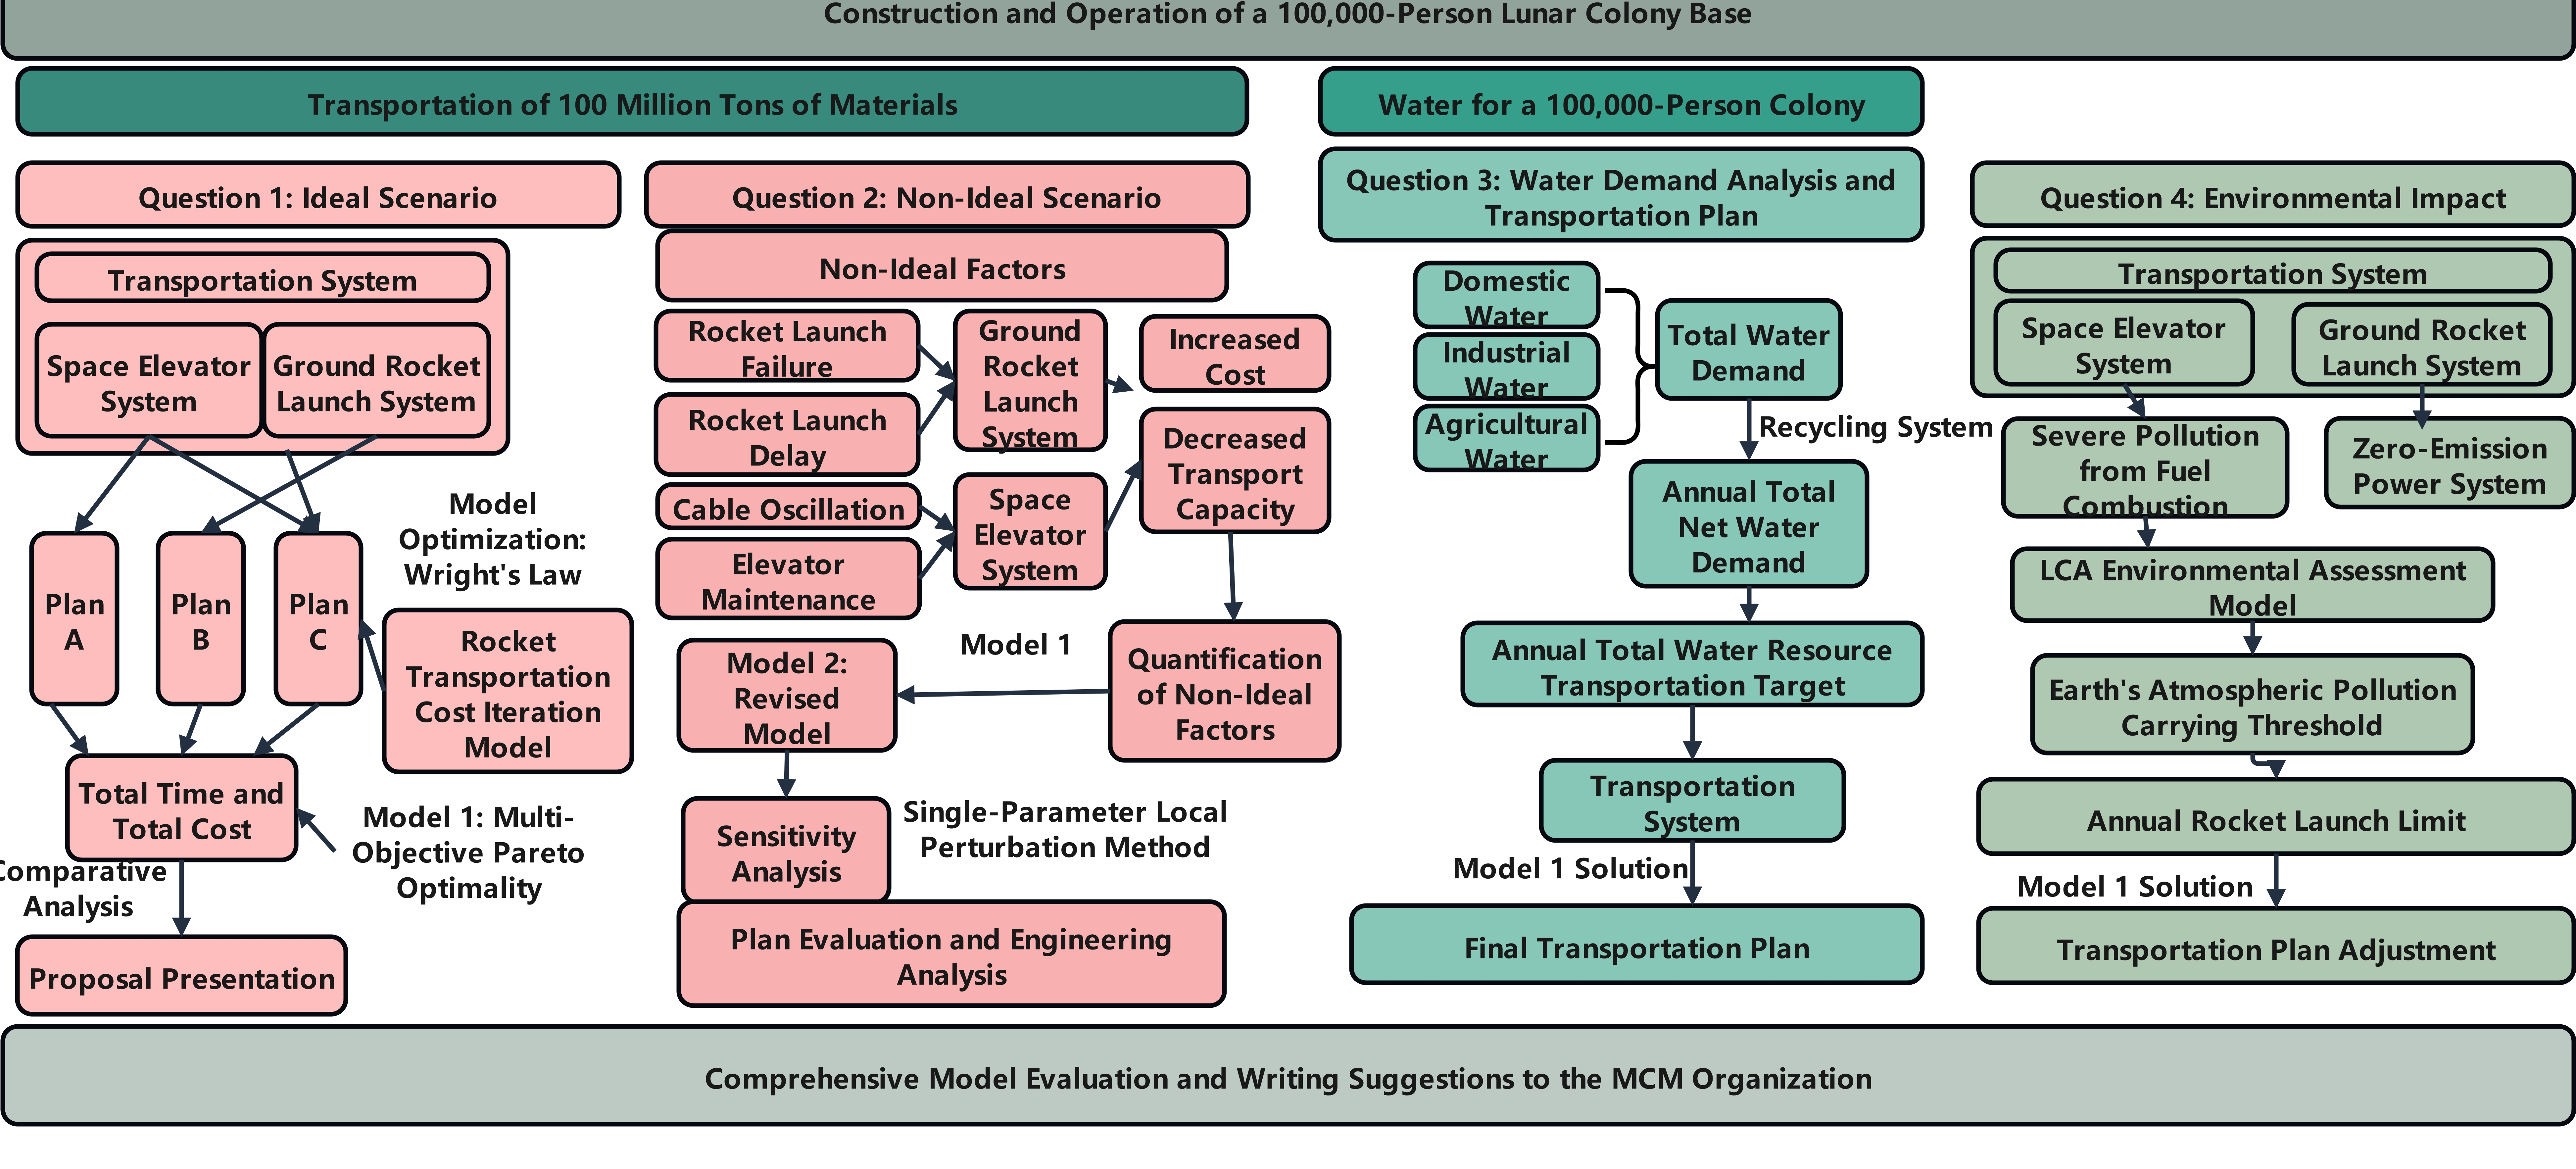
\includegraphics[width=1.00\textwidth]{../figures/ourwork.jpg}
  \caption{Our Work}
  \label{fig:Our Work}
\end{figure}
\FloatBarrier


